% Options for packages loaded elsewhere
\PassOptionsToPackage{unicode}{hyperref}
\PassOptionsToPackage{hyphens}{url}
\PassOptionsToPackage{dvipsnames,svgnames,x11names}{xcolor}
%
\documentclass[
  a4paper,
  DIV=11,
  numbers=noendperiod]{scrreprt}

\usepackage{amsmath,amssymb}
\usepackage{iftex}
\ifPDFTeX
  \usepackage[T1]{fontenc}
  \usepackage[utf8]{inputenc}
  \usepackage{textcomp} % provide euro and other symbols
\else % if luatex or xetex
  \usepackage{unicode-math}
  \defaultfontfeatures{Scale=MatchLowercase}
  \defaultfontfeatures[\rmfamily]{Ligatures=TeX,Scale=1}
\fi
\usepackage{lmodern}
\ifPDFTeX\else  
    % xetex/luatex font selection
\fi
% Use upquote if available, for straight quotes in verbatim environments
\IfFileExists{upquote.sty}{\usepackage{upquote}}{}
\IfFileExists{microtype.sty}{% use microtype if available
  \usepackage[]{microtype}
  \UseMicrotypeSet[protrusion]{basicmath} % disable protrusion for tt fonts
}{}
\makeatletter
\@ifundefined{KOMAClassName}{% if non-KOMA class
  \IfFileExists{parskip.sty}{%
    \usepackage{parskip}
  }{% else
    \setlength{\parindent}{0pt}
    \setlength{\parskip}{6pt plus 2pt minus 1pt}}
}{% if KOMA class
  \KOMAoptions{parskip=half}}
\makeatother
\usepackage{xcolor}
\setlength{\emergencystretch}{3em} % prevent overfull lines
\setcounter{secnumdepth}{5}
% Make \paragraph and \subparagraph free-standing
\ifx\paragraph\undefined\else
  \let\oldparagraph\paragraph
  \renewcommand{\paragraph}[1]{\oldparagraph{#1}\mbox{}}
\fi
\ifx\subparagraph\undefined\else
  \let\oldsubparagraph\subparagraph
  \renewcommand{\subparagraph}[1]{\oldsubparagraph{#1}\mbox{}}
\fi

\usepackage{color}
\usepackage{fancyvrb}
\newcommand{\VerbBar}{|}
\newcommand{\VERB}{\Verb[commandchars=\\\{\}]}
\DefineVerbatimEnvironment{Highlighting}{Verbatim}{commandchars=\\\{\}}
% Add ',fontsize=\small' for more characters per line
\usepackage{framed}
\definecolor{shadecolor}{RGB}{241,243,245}
\newenvironment{Shaded}{\begin{snugshade}}{\end{snugshade}}
\newcommand{\AlertTok}[1]{\textcolor[rgb]{0.68,0.00,0.00}{#1}}
\newcommand{\AnnotationTok}[1]{\textcolor[rgb]{0.37,0.37,0.37}{#1}}
\newcommand{\AttributeTok}[1]{\textcolor[rgb]{0.40,0.45,0.13}{#1}}
\newcommand{\BaseNTok}[1]{\textcolor[rgb]{0.68,0.00,0.00}{#1}}
\newcommand{\BuiltInTok}[1]{\textcolor[rgb]{0.00,0.23,0.31}{#1}}
\newcommand{\CharTok}[1]{\textcolor[rgb]{0.13,0.47,0.30}{#1}}
\newcommand{\CommentTok}[1]{\textcolor[rgb]{0.37,0.37,0.37}{#1}}
\newcommand{\CommentVarTok}[1]{\textcolor[rgb]{0.37,0.37,0.37}{\textit{#1}}}
\newcommand{\ConstantTok}[1]{\textcolor[rgb]{0.56,0.35,0.01}{#1}}
\newcommand{\ControlFlowTok}[1]{\textcolor[rgb]{0.00,0.23,0.31}{#1}}
\newcommand{\DataTypeTok}[1]{\textcolor[rgb]{0.68,0.00,0.00}{#1}}
\newcommand{\DecValTok}[1]{\textcolor[rgb]{0.68,0.00,0.00}{#1}}
\newcommand{\DocumentationTok}[1]{\textcolor[rgb]{0.37,0.37,0.37}{\textit{#1}}}
\newcommand{\ErrorTok}[1]{\textcolor[rgb]{0.68,0.00,0.00}{#1}}
\newcommand{\ExtensionTok}[1]{\textcolor[rgb]{0.00,0.23,0.31}{#1}}
\newcommand{\FloatTok}[1]{\textcolor[rgb]{0.68,0.00,0.00}{#1}}
\newcommand{\FunctionTok}[1]{\textcolor[rgb]{0.28,0.35,0.67}{#1}}
\newcommand{\ImportTok}[1]{\textcolor[rgb]{0.00,0.46,0.62}{#1}}
\newcommand{\InformationTok}[1]{\textcolor[rgb]{0.37,0.37,0.37}{#1}}
\newcommand{\KeywordTok}[1]{\textcolor[rgb]{0.00,0.23,0.31}{#1}}
\newcommand{\NormalTok}[1]{\textcolor[rgb]{0.00,0.23,0.31}{#1}}
\newcommand{\OperatorTok}[1]{\textcolor[rgb]{0.37,0.37,0.37}{#1}}
\newcommand{\OtherTok}[1]{\textcolor[rgb]{0.00,0.23,0.31}{#1}}
\newcommand{\PreprocessorTok}[1]{\textcolor[rgb]{0.68,0.00,0.00}{#1}}
\newcommand{\RegionMarkerTok}[1]{\textcolor[rgb]{0.00,0.23,0.31}{#1}}
\newcommand{\SpecialCharTok}[1]{\textcolor[rgb]{0.37,0.37,0.37}{#1}}
\newcommand{\SpecialStringTok}[1]{\textcolor[rgb]{0.13,0.47,0.30}{#1}}
\newcommand{\StringTok}[1]{\textcolor[rgb]{0.13,0.47,0.30}{#1}}
\newcommand{\VariableTok}[1]{\textcolor[rgb]{0.07,0.07,0.07}{#1}}
\newcommand{\VerbatimStringTok}[1]{\textcolor[rgb]{0.13,0.47,0.30}{#1}}
\newcommand{\WarningTok}[1]{\textcolor[rgb]{0.37,0.37,0.37}{\textit{#1}}}

\providecommand{\tightlist}{%
  \setlength{\itemsep}{0pt}\setlength{\parskip}{0pt}}\usepackage{longtable,booktabs,array}
\usepackage{calc} % for calculating minipage widths
% Correct order of tables after \paragraph or \subparagraph
\usepackage{etoolbox}
\makeatletter
\patchcmd\longtable{\par}{\if@noskipsec\mbox{}\fi\par}{}{}
\makeatother
% Allow footnotes in longtable head/foot
\IfFileExists{footnotehyper.sty}{\usepackage{footnotehyper}}{\usepackage{footnote}}
\makesavenoteenv{longtable}
\usepackage{graphicx}
\makeatletter
\def\maxwidth{\ifdim\Gin@nat@width>\linewidth\linewidth\else\Gin@nat@width\fi}
\def\maxheight{\ifdim\Gin@nat@height>\textheight\textheight\else\Gin@nat@height\fi}
\makeatother
% Scale images if necessary, so that they will not overflow the page
% margins by default, and it is still possible to overwrite the defaults
% using explicit options in \includegraphics[width, height, ...]{}
\setkeys{Gin}{width=\maxwidth,height=\maxheight,keepaspectratio}
% Set default figure placement to htbp
\makeatletter
\def\fps@figure{htbp}
\makeatother

\KOMAoption{captions}{tableheading}
\makeatletter
\@ifpackageloaded{bookmark}{}{\usepackage{bookmark}}
\makeatother
\makeatletter
\@ifpackageloaded{caption}{}{\usepackage{caption}}
\AtBeginDocument{%
\ifdefined\contentsname
  \renewcommand*\contentsname{Table of contents}
\else
  \newcommand\contentsname{Table of contents}
\fi
\ifdefined\listfigurename
  \renewcommand*\listfigurename{List of Figures}
\else
  \newcommand\listfigurename{List of Figures}
\fi
\ifdefined\listtablename
  \renewcommand*\listtablename{List of Tables}
\else
  \newcommand\listtablename{List of Tables}
\fi
\ifdefined\figurename
  \renewcommand*\figurename{Figure}
\else
  \newcommand\figurename{Figure}
\fi
\ifdefined\tablename
  \renewcommand*\tablename{Table}
\else
  \newcommand\tablename{Table}
\fi
}
\@ifpackageloaded{float}{}{\usepackage{float}}
\floatstyle{ruled}
\@ifundefined{c@chapter}{\newfloat{codelisting}{h}{lop}}{\newfloat{codelisting}{h}{lop}[chapter]}
\floatname{codelisting}{Listing}
\newcommand*\listoflistings{\listof{codelisting}{List of Listings}}
\makeatother
\makeatletter
\makeatother
\makeatletter
\@ifpackageloaded{caption}{}{\usepackage{caption}}
\@ifpackageloaded{subcaption}{}{\usepackage{subcaption}}
\makeatother
\ifLuaTeX
\usepackage[bidi=basic]{babel}
\else
\usepackage[bidi=default]{babel}
\fi
\babelprovide[main,import]{english}
% get rid of language-specific shorthands (see #6817):
\let\LanguageShortHands\languageshorthands
\def\languageshorthands#1{}
\ifLuaTeX
  \usepackage{selnolig}  % disable illegal ligatures
\fi
\IfFileExists{bookmark.sty}{\usepackage{bookmark}}{\usepackage{hyperref}}
\IfFileExists{xurl.sty}{\usepackage{xurl}}{} % add URL line breaks if available
\urlstyle{same} % disable monospaced font for URLs
\hypersetup{
  pdftitle={Potential Theory},
  pdfauthor={Dr.~Ralph-Uwe Börner},
  pdflang={en},
  colorlinks=true,
  linkcolor={blue},
  filecolor={Maroon},
  citecolor={Blue},
  urlcolor={Blue},
  pdfcreator={LaTeX via pandoc}}

\title{Potential Theory}
\author{Dr.~Ralph-Uwe Börner}
\date{2023-12-07}

\begin{document}
\maketitle
\renewcommand*\contentsname{Table of contents}
{
\hypersetup{linkcolor=}
\setcounter{tocdepth}{2}
\tableofcontents
}
\bookmarksetup{startatroot}

\chapter{Introduction}\label{introduction}

This is work in progress!

\part{Prerequisites}

\part{Mathematical foundations}

\chapter{Fields}\label{fields}

\section{Potential fields}\label{potential-fields}

\section{Density}\label{density}

\section{Point sources}\label{point-sources}

\section{Solution of the Laplace and Poisson
equations}\label{solution-of-the-laplace-and-poisson-equations}

We consider the second-order differential equations

\[
\dv[2]{y}{x} = 0
\]

(\emph{Laplace equation}) and

\[
\dv[2]{y}{x} = -4\cos(4x) - 8 \sin(8 x)
\]

(\emph{Poisson equation}) for \(x \in [0, 1]\) subject to the boundary
conditions \(y(0)=1\) and \(y(1)=0\).

To obtain the solution to the above PDEs, we employ the \texttt{Python}
package \texttt{sympy}, which is a powerful library for symbolic
mathematics.

Symbolic functions which depend on symbolic variables have to be defined
with the function \texttt{Function}.

The solution of the differential equations can be obtained by a call to
the \texttt{dsolve} function.

The signature of the function can be understood as follows:

\begin{itemize}
\tightlist
\item
  Solve the symbolic equation given by the expressions
  \texttt{eq\_poisson} and \texttt{eq\_laplace}, resp.
\item
  The desired solution is \texttt{y(x)}
\item
  Boundary conditions can be enforced by the values following the
  keyword \texttt{ics}. In the example, \texttt{y(0)=1} and
  \texttt{y(1)=0}.
\end{itemize}

\begin{Shaded}
\begin{Highlighting}[]
\ImportTok{from}\NormalTok{ sympy }\ImportTok{import}\NormalTok{ Function, dsolve, diff, cos, sin}
\ImportTok{from}\NormalTok{ sympy.abc }\ImportTok{import}\NormalTok{ x}
\ImportTok{from}\NormalTok{ sympy.plotting }\ImportTok{import}\NormalTok{ plot, PlotGrid}
\ImportTok{import}\NormalTok{ matplotlib.pyplot }\ImportTok{as}\NormalTok{ plt}
\CommentTok{\# plt.style.use(\textquotesingle{}fivethirtyeight\textquotesingle{})}

\NormalTok{y }\OperatorTok{=}\NormalTok{ Function(}\StringTok{\textquotesingle{}y\textquotesingle{}}\NormalTok{)}
\NormalTok{eq\_poisson }\OperatorTok{=}\NormalTok{ diff(y(x), x, }\DecValTok{2}\NormalTok{) }\OperatorTok{+} \DecValTok{4} \OperatorTok{*}\NormalTok{ cos(}\DecValTok{4} \OperatorTok{*}\NormalTok{ x) }\OperatorTok{+} \DecValTok{8} \OperatorTok{*}\NormalTok{ sin(}\DecValTok{8} \OperatorTok{*}\NormalTok{ x)}
\NormalTok{eq\_laplace }\OperatorTok{=}\NormalTok{ diff(y(x), x, }\DecValTok{2}\NormalTok{)}
\NormalTok{result\_poisson }\OperatorTok{=}\NormalTok{ dsolve(eq\_poisson, y(x), ics}\OperatorTok{=}\NormalTok{\{y(}\DecValTok{0}\NormalTok{): }\DecValTok{1}\NormalTok{, y(}\DecValTok{1}\NormalTok{): }\DecValTok{0}\NormalTok{\})}
\NormalTok{result\_laplace }\OperatorTok{=}\NormalTok{ dsolve(eq\_laplace, y(x), ics}\OperatorTok{=}\NormalTok{\{y(}\DecValTok{0}\NormalTok{): }\DecValTok{1}\NormalTok{, y(}\DecValTok{1}\NormalTok{): }\DecValTok{0}\NormalTok{\})}
\NormalTok{p1 }\OperatorTok{=}\NormalTok{ plot(result\_poisson.rhs, (x, }\DecValTok{0}\NormalTok{, }\DecValTok{1}\NormalTok{), }
\NormalTok{      ylim}\OperatorTok{=}\NormalTok{(}\OperatorTok{{-}}\FloatTok{0.2}\NormalTok{, }\FloatTok{1.2}\NormalTok{), }
\NormalTok{      ylabel}\OperatorTok{=}\StringTok{\textquotesingle{}y(x)\textquotesingle{}}\NormalTok{, }
\NormalTok{      axis\_center}\OperatorTok{=}\StringTok{\textquotesingle{}auto\textquotesingle{}}\NormalTok{,}
\NormalTok{      show}\OperatorTok{=}\VariableTok{False}\NormalTok{,}
\NormalTok{      title}\OperatorTok{=}\StringTok{\textquotesingle{}Poisson equation\textquotesingle{}}\NormalTok{)}\OperatorTok{;}
\NormalTok{p2 }\OperatorTok{=}\NormalTok{ plot(result\_laplace.rhs, (x, }\DecValTok{0}\NormalTok{, }\DecValTok{1}\NormalTok{), }
\NormalTok{      ylim}\OperatorTok{=}\NormalTok{(}\OperatorTok{{-}}\FloatTok{0.2}\NormalTok{, }\FloatTok{1.2}\NormalTok{), }
\NormalTok{      ylabel}\OperatorTok{=}\StringTok{\textquotesingle{}y(x)\textquotesingle{}}\NormalTok{, }
\NormalTok{      axis\_center}\OperatorTok{=}\StringTok{\textquotesingle{}auto\textquotesingle{}}\NormalTok{,}
\NormalTok{      show}\OperatorTok{=}\VariableTok{False}\NormalTok{,}
\NormalTok{      title}\OperatorTok{=}\StringTok{\textquotesingle{}Laplace equation\textquotesingle{}}\NormalTok{)}\OperatorTok{;}
\NormalTok{PlotGrid(}\DecValTok{1}\NormalTok{, }\DecValTok{2}\NormalTok{, p1, p2, size}\OperatorTok{=}\NormalTok{(}\DecValTok{7}\NormalTok{,}\DecValTok{3}\NormalTok{))}\OperatorTok{;}
\end{Highlighting}
\end{Shaded}

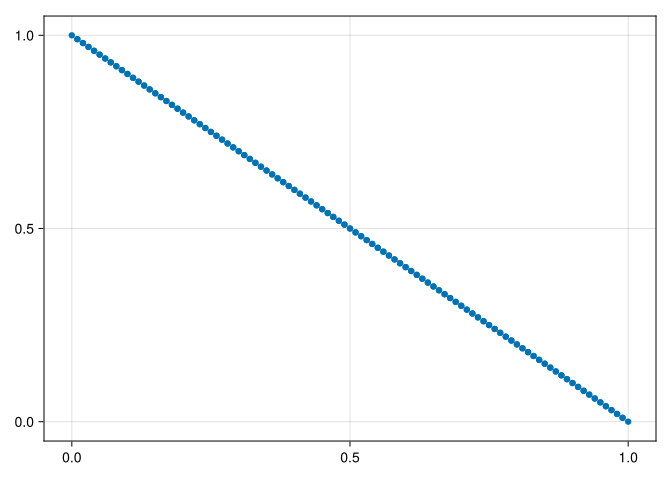
\includegraphics{fields_files/figure-pdf/cell-2-output-1.pdf}

\section{What can be observed in the 1-D
case?}\label{what-can-be-observed-in-the-1-d-case}

\begin{itemize}
\tightlist
\item
  The solution of the \emph{Laplace equation} does not exhibit local
  extrema

  \begin{itemize}
  \tightlist
  \item
    It has no curvature
  \end{itemize}
\item
  The solution of the \emph{Poisson equation} has local minima and
  maxima

  \begin{itemize}
  \tightlist
  \item
    Its extrema might get larger or smaller than those of the Dirichlet
    values at the boundary
  \end{itemize}
\end{itemize}

\part{Newton potential}

\chapter{Point Mass}\label{point-mass}

\chapter{Poisson Equation}\label{poisson-equation}

\chapter{Mass distribution}\label{mass-distribution}

\chapter{Newton's Shell Theorem}\label{newtons-shell-theorem}

\chapter{Legendre Polynomials}\label{legendre-polynomials}

\chapter{Circular Disc}\label{circular-disc}

\chapter{Geophysical Application}\label{geophysical-application}

\section{Planetary density models}\label{planetary-density-models}

\section{Bouguer reduction}\label{bouguer-reduction}

\section{Gravitational attraction of a spherical
body}\label{gravitational-attraction-of-a-spherical-body}

\part{Two-dimensional problems}

\chapter{2-D mass distributions}\label{d-mass-distributions}

We consider an elongated mass with a lateral extension that is much
larger than any profile crossing it at a right angle. Those mass
distributions are invariant along one of the horizontal Cartesian axes.

If we consider the \(x\)-direction as the \emph{strike direction}, then
we can restrict our derivations to a single arbitrary \(x\)-plane, e.g.,
the plane \(x=0\). Thus, any field configuration observed in the
\(y-z\)-plane is invariant with respect to a shift in the
\(x\)-direction.

First, we derive an expression for the gravitational attraction of a
simple horizontal line, e.g., an infinite wire.

Next, we make the transition to a polar coordinate system which is much
better suited for the purpose of numerical implementation. To this end,
we follow the work of @hubbert1948 and @talwani1959.

\section{A horizontal straight line of
mass}\label{a-horizontal-straight-line-of-mass}

As usual, we depart from a simple geometry. Later we integrate over a
cross section of arbitrary shape to obtain the potential and
gravitational attraction of elongated bodies.

For an \(x\)-directed straight wire of density \(\rho_L\) we obtain for
the gravitational attraction in the plane \(x=0\)

\begin{equation}\phantomsection\label{eq-attraction-line}{
\mathbf g(0, y, z) = f \rho_L \int\limits_{x'=-\infty}^\infty \nabla \frac{1}{{x'}^2 + (y - y')^2 + (z - z')^2} \mathrm{d}x'
}\end{equation}

\emph{SymPy} is a Python library for symbolic mathematics. It yields the
following result for the \(z\)-component of \(\mathbf g\), i.e.,

\[
g_z(0, y, z) = f \rho_L \int\limits_{x'=-\infty}^\infty \frac{\partial}{\partial z} \frac{1}{{x'}^2 + (y - y')^2 + (z - z')^2} \mathrm{d}x'
\]

\begin{Shaded}
\begin{Highlighting}[]
\NormalTok{x, y, z, xprime, yprime, zprime, f, rho\_L }\OperatorTok{=}\NormalTok{ symbols(}\StringTok{\textquotesingle{}x y z xprime yprime zprime f rho\_L\textquotesingle{}}\NormalTok{, real}\OperatorTok{=}\VariableTok{True}\NormalTok{)}
\NormalTok{g\_z }\OperatorTok{=}\NormalTok{ integrate(f }\OperatorTok{*}\NormalTok{ rho\_L }\OperatorTok{*}\NormalTok{ diff(}\DecValTok{1} \OperatorTok{/}\NormalTok{ sqrt(xprime}\OperatorTok{**}\DecValTok{2} \OperatorTok{+}\NormalTok{ (y }\OperatorTok{{-}}\NormalTok{ yprime)}\OperatorTok{**}\DecValTok{2} \OperatorTok{+}\NormalTok{ (z }\OperatorTok{{-}}\NormalTok{ zprime)}\OperatorTok{**}\DecValTok{2}\NormalTok{), z), (xprime, }\OperatorTok{{-}}\NormalTok{oo, oo))}
\CommentTok{\# display(simplify(g\_z))}
\NormalTok{display(Math(}\SpecialStringTok{f\textquotesingle{} g\_z(y,z) = }\SpecialCharTok{\{}\NormalTok{latex(simplify(g\_z))}\SpecialCharTok{\}}\SpecialStringTok{\textquotesingle{}}\NormalTok{))}
\end{Highlighting}
\end{Shaded}

$\displaystyle  g_z(y,z) = - \frac{2 f \rho_{L} \left(z - {z}'\right)}{\left(y - {y}'\right)^{2} + \left(z - {z}'\right)^{2}}$

We recognize that

\[
g_z(y,z) = - 2 f \rho_L \frac{z - z'}{(y - y')^2 + (z - z')^2}
\]

The interesting point is here that the numerator is the derivative of
the denominator, i.e.,

\[
f'(z) = 2(z - z')
\]

and

\[
f(z) = (y - y')^2 + (z - z')^2
\]

With the \emph{logarithmic derivative}

\[
\int \frac{f'(z)}{f(z)} \mathrm dz = \ln f(z) + C
\]

we obtain the \emph{logarithmic potential} by integrating with respect
to \(z\), which yields

\[
V(y,z) = -2 f \rho_L \ln \sqrt{(y - y')^2 + (z - z')^2} + C
\]

or

\[ \ln r^2 = 2 \ln r \] \[ \ln r = -\ln \frac{1}{r} \]

\[
V(y,z) = 2 f \rho_L \ln \frac{1}{r}
\]

Note that we set \(C = 0 = 2 f \rho_L \ln 1\).

Thus, with a proper choice of \(C\), we can shift the potential such
that \(V\) takes a desired value at a given distance from the line of
mass. In our case, the potential is zero at the \emph{finite} distance
of \(r=1\), and not at infinity as it would be the case for finite
bodies where \(V \sim 1/r\). In the 2-D case, the masses extend to
infinity.

\begin{Shaded}
\begin{Highlighting}[]
\NormalTok{V }\OperatorTok{=} \OperatorTok{{-}}\DecValTok{2} \OperatorTok{*}\NormalTok{ f }\OperatorTok{*}\NormalTok{ rho\_L }\OperatorTok{*}\NormalTok{ log(sqrt((y}\OperatorTok{{-}}\NormalTok{ yprime)}\OperatorTok{**}\DecValTok{2} \OperatorTok{+}\NormalTok{ (z }\OperatorTok{{-}}\NormalTok{ zprime)}\OperatorTok{**}\DecValTok{2}\NormalTok{))}
\CommentTok{\# display(V)}
\NormalTok{plot(V.subs([(f, }\DecValTok{1}\NormalTok{), (rho\_L, }\DecValTok{1}\NormalTok{), (z, }\DecValTok{0}\NormalTok{), (zprime, }\DecValTok{5}\NormalTok{), (yprime, }\DecValTok{0}\NormalTok{)]),}
\NormalTok{  (y, }\OperatorTok{{-}}\DecValTok{5}\NormalTok{, }\DecValTok{5}\NormalTok{), size}\OperatorTok{=}\NormalTok{(}\DecValTok{4}\NormalTok{, }\DecValTok{3}\NormalTok{),}
\NormalTok{  xlabel}\OperatorTok{=}\StringTok{\textquotesingle{}y\textquotesingle{}}\NormalTok{, ylabel}\OperatorTok{=}\VerbatimStringTok{r\textquotesingle{}$V(y)$\textquotesingle{}}\NormalTok{, ylim}\OperatorTok{=}\NormalTok{(}\OperatorTok{{-}}\DecValTok{4}\NormalTok{, }\OperatorTok{{-}}\DecValTok{3}\NormalTok{), xlim}\OperatorTok{=}\NormalTok{(}\OperatorTok{{-}}\DecValTok{5}\NormalTok{, }\DecValTok{5}\NormalTok{), axis\_center}\OperatorTok{=}\NormalTok{(}\OperatorTok{{-}}\DecValTok{5}\NormalTok{, }\OperatorTok{{-}}\DecValTok{4}\NormalTok{))}
\end{Highlighting}
\end{Shaded}

\begin{figure}[H]

{\centering 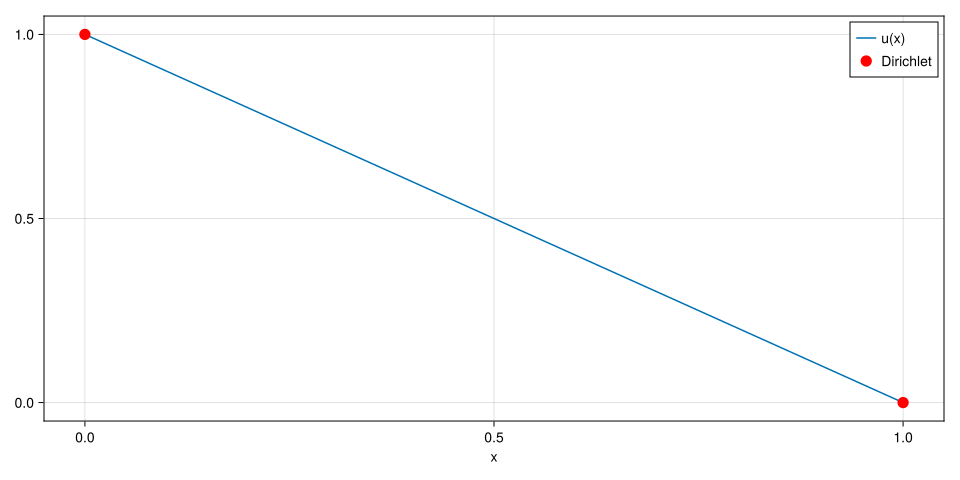
\includegraphics{line_of_mass_files/figure-pdf/cell-4-output-1.pdf}

}

\caption{Potential \(V\) of an infinite wire at \(y=0\) and \(z=5\),
\(f \rho_L = 1\).}

\end{figure}%

\begin{Shaded}
\begin{Highlighting}[]
\NormalTok{plot(g\_z.subs([(f, }\DecValTok{1}\NormalTok{), (rho\_L, }\DecValTok{1}\NormalTok{), (z, }\DecValTok{0}\NormalTok{), (zprime, }\DecValTok{5}\NormalTok{), (yprime, }\DecValTok{0}\NormalTok{)]), }
\NormalTok{  (y, }\OperatorTok{{-}}\DecValTok{5}\NormalTok{, }\DecValTok{5}\NormalTok{), size}\OperatorTok{=}\NormalTok{(}\DecValTok{4}\NormalTok{, }\DecValTok{3}\NormalTok{),}
\NormalTok{  xlabel}\OperatorTok{=}\StringTok{\textquotesingle{}y\textquotesingle{}}\NormalTok{, ylabel}\OperatorTok{=}\VerbatimStringTok{r\textquotesingle{}$g\_z(y)$\textquotesingle{}}\NormalTok{, axis\_center}\OperatorTok{=}\NormalTok{(}\OperatorTok{{-}}\DecValTok{5}\NormalTok{, }\DecValTok{0}\NormalTok{), ylim}\OperatorTok{=}\NormalTok{(}\DecValTok{0}\NormalTok{,}\FloatTok{0.5}\NormalTok{), xlim}\OperatorTok{=}\NormalTok{(}\OperatorTok{{-}}\DecValTok{5}\NormalTok{,}\DecValTok{5}\NormalTok{))}
\end{Highlighting}
\end{Shaded}

\begin{figure}[H]

{\centering 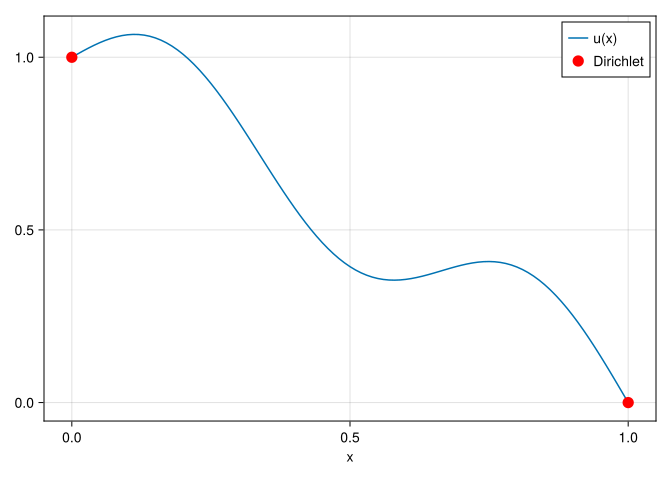
\includegraphics{line_of_mass_files/figure-pdf/cell-5-output-1.pdf}

}

\caption{Vertical attraction \(g_z\) of an infinite wire at \(y=0\) and
\(z=5\), \(f \rho_L = 1\).}

\end{figure}%

\section{Attraction of a plane
lamina}\label{attraction-of-a-plane-lamina}

The vertical component of attraction due to an element of area
\(\mathrm{d}S\) on an infinite horizontal plane lamina with density
\(\rho\) bounded by the planes \(z\) and \(z+\mathrm{d}z\) is \[
\mathrm{d}g = f \rho \mathrm{d}z \mathrm{d}\Omega 
\] where \(\mathrm{d}\Omega\) is the solid angle subtended at the origin
by the area \(\mathrm{d}S\).

\includegraphics{images/hubbert_01.png}

It holds \[
\mathrm{d}\Omega = \frac{\mathrm{d}S \sin \alpha}{r^{2}.}
\]

If we now consider a finite area \(S\) of arbitrary shape, the
attraction at the origin due to the enclosed mass will be \[
g = f \mathrm{d}z \int _{S} \rho \, \mathrm{d}\Omega 
\] or, if \(\rho\) is constant over \(S\), this simplifies to \[
g = f \rho \Omega \mathrm{d}z.
\] For a given solid angle \(\Omega\), the attraction of the matter
enclosed between two horizontal planes at \(z=z_{1}\) and \(z=z_{2}\)
will be obtained by integrating \[
g = f \Omega \int_{z_{1}}^{z_{2}} \rho \, \mathrm{d}z 
\] and if \(\rho=\mathrm{const.}\) this becomes \[
g = f \rho \Omega (z_{2} - z_{1})
\] For the infinite horizontal plane the solid angle is \(2 \pi\), such
that the attraction of an infinite plate will be \[
g = 2 \pi f \rho (z_{2} - z_{1})
\] which is the vertical attraction of the Bouguer plate of thickness
\(z_{2} - z_{1}\) and density \(\rho\).

\section{\texorpdfstring{The \(\mathrm{d}\Theta\mathrm{d}z\)
solenoid}{The \textbackslash mathrm\{d\}\textbackslash Theta\textbackslash mathrm\{d\}z solenoid}}\label{the-mathrmdthetamathrmdz-solenoid}

First, we consider the attraction at the origin which will result from a
narrow linear strip of infinite length parallel to the \(x\)-axis. Such
a strip will be defined by the area on the plane \(z=\mathrm{const.}\)
lying between two inclined planes which intersect on the \(x\)-axis and
make with the \(y\)-axis the angles of \(\Theta\) and
\(\Theta + \mathrm{d}\Theta\).

\includegraphics{images/hubbert_02.png}

The attraction of this strip is proportional to the solid angle
subtended by it at the origin. The solid angle \(\mathrm{d}\Omega\)
between two planes intersecting at an angle \(\mathrm{d}\Theta\) will
bear the same ratio to the total solid angle which the plane angle
\(\mathrm{d}\Theta\) bears to the total plane angle. The total solid
angle is the ratio of the surface area of a sphere to the square of its
radius, or \(4 \pi\), and the total plane angle is \(2 \pi\). Thus \[
\frac{\mathrm{d}\Omega}{4 \pi} = \frac{\mathrm{d}\Theta}{2 \pi}
\] or \[
\mathrm{d}\Omega = 2 \mathrm{d}\Theta.
\] Introducing this to the result obtained above gives \[
\mathrm{d}g = 2 f \rho \mathrm{d}\Theta \mathrm{d}z
\] which is the \emph{fundamental differential equation of the
attraction of a two-dimensional mass}. The intersection of the two
planes \(\Theta\) and \(\Theta + \mathrm{d}\Theta\) with the planes
\(z\) and \(z+\mathrm{d}z\) defines an elementary prism or solenoid of
infinite length and cross-section \(\mathrm{d}\Theta\mathrm{d}z\). For a
finite area in the plane of integration \[
g = 2 f \iint \rho \mathrm{d}\Theta \mathrm{d}z
\] Around an elementary prism \(\mathrm{d}\Theta\mathrm{d}z\) bounded by
the lines \(\Theta\) and \(\Theta + \mathrm{d}\Theta\), and \(z\) and
\(z+\mathrm{d}z\), consider the line integral
\(\oint \Theta \mathrm{d}z\). Traversing the circuit in
counter-clockwise direction, the resulting integral will be \[
\oint \Theta \mathrm{d}z = 0 + (\Theta + \mathrm{d}\Theta)\mathrm{d}z + 0 - \Theta \mathrm{d}z = \mathrm{d}\Theta \mathrm{d}z.
\] Over a finite area \(S\) we may obtain
\(\iint \mathrm{d}\Theta \mathrm{d}z\) by \[
\iint_{S} \mathrm{d}\Theta \mathrm{d}z = \iint_{S} \left[\oint \Theta \mathrm{d}z \right].
\] When a separate line integral is taken around each of the elementary
prisms of the area, each interior part is traversed twice, whereas the
exterior parts are traversed but once and always in the same sense.
Consequently, \[
\iint_{S} \mathrm{d}\Theta \mathrm{d}z = \oint_{s} \Theta \mathrm{d}z.
\] The attraction of a finite mass of constant density is obtained by \[
g = 2 f \rho \oint_{s} \Theta \mathrm{d}z.
\] ---

\chapter{Gravitational attraction of a
prism}\label{gravitational-attraction-of-a-prism}

\section{Problem description}\label{problem-description}

Recall that the vertical component of the gravitational attraction
caused by an elongated prismatic body of cross section \(S\) is

\[
g_z(x,z) = \frac{\partial}{\partial z}V(x,z) = -2 f \Delta \rho \int\limits_S \frac{(z - z')\, dx' \,dz'}{(x-x')^2 + (z-z')^2}.
\]

If the point of observation is at the origin, we obtain

\[
g_z(0,0) = \frac{\partial}{\partial z}V(0,0) = 2 f \Delta \rho \int\limits_S \frac{z\, dx \, dz}{x^2 + z^2}.
\]

It can be shown that this surface integral can be equivalently replaced
by a line integral taken along the periphery of \(S\).

\section{Line integral}\label{line-integral}

The Stokes theorem~states that, for any vector field
\(\mathbf A = (A_x, 0, A_z)^\top\) there holds

\[
\int\limits_S (\nabla \times \mathbf A) \cdot d\mathbf s = \oint\limits_C \mathbf A \cdot d\mathbf \ell,
\]

where \(d\mathbf\ell = \mathbf e_x dx + \mathbf e_z dz\) is the oriented
line element tangential to the curve \(C\), and
\(d\mathbf s = dx \,dz \, \mathbf e_y\) the oriented surface element
normal to the cross section \(S\). It follows by inspection that

\[
\partial_z A_x - \partial_x A_z = 2 f \Delta \rho \frac{z}{x^2 + z^2}
\]

such that, after making the \emph{ansatz} (@zhou2008)

\[
A_x = 0, \qquad A_z = -2 f \Delta\rho \, z \left(\frac{1}{z} \, \tan^{-1}\frac{x}{z}\right) = -2 f \Delta \rho \, \theta
\]

The angle \(\theta\) is taken from the positive \(x\)-axis towards the
positive \(z\)-axis.

@talwani1959 have shown that the vertical component of the gravitational
attraction of a two-dimensional prismatic body is, at the origin, equal
to

\[
g_z(0, 0) = 2 f \Delta \rho \oint\limits_C z \, d\theta,
\]

i.e., a line integral taken along its periphery.

The following sketch illustrates the situation (taken from the original
Talwani paper).

\includegraphics{index_files/mediabag/Talwani-2D.png}

Let \(ABCDEF\) be a given polygon with \(n\) sides and let \(P\) be the
point at which the gravitational attraction due to this body has to be
computed.

Further, let \(z\) be defined positive downwards and let \(\theta\) be
measured from the positive \(x\)-axis towards the positive \(z\)-axis.

Let us evaluate the integral \(\oint z\, d\theta\) for the above
polygon.

We consider here the contribution from the side \(BC\). The remaining
sides have to be added to obtain the total gravitational attraction of
the complete prism.

At the point \(Q\) the line \(BC\) meets the \(x\)-axis at an angle
\(\phi_i\).

Let \(PQ = a_i\). For any arbitrary point \(R = R(x,z)\) on the side
\(BC\) there hold the two equivalent equations

\[
z = x \tan\theta
\]

and

\[
z = (x - a_i) \tan\phi_i.
\]

After eliminating \(x\) we obtain an expression for \(z = z(\theta)\):

\[
z = \frac{a_i \tan\phi_i \tan\theta}{\tan\phi_i - \tan\theta}
\]

The contribution of the segment \(BC\) to the above line integral can
now be rewritten as

\[
\int_{BC} z \, d\theta = \int\limits_B^C \frac{a_i \tan\phi_i \tan\theta}{\tan\phi_i - \tan\theta} \, d\theta =: Z_i.
\]

The vertical component of the gravitational attraction is

\[
g_z(0, 0) = 2 f \Delta \rho \sum_{i=1}^n Z_i.
\]

It remains to solve the integral in the expression for \(Z_i\). To this
end, we use \texttt{Sympy}.

\section{Implementation}\label{implementation}

\begin{Shaded}
\begin{Highlighting}[]
\NormalTok{a, x, z, phi, theta, Z }\OperatorTok{=}\NormalTok{ symbols(}\StringTok{\textquotesingle{}a x z phi theta Z\textquotesingle{}}\NormalTok{, real}\OperatorTok{=}\VariableTok{True}\NormalTok{)}
\NormalTok{Z }\OperatorTok{=}\NormalTok{ solve([tan(theta) }\OperatorTok{*}\NormalTok{ x }\OperatorTok{{-}}\NormalTok{ z, (x }\OperatorTok{{-}}\NormalTok{ a) }\OperatorTok{*}\NormalTok{ tan(phi) }\OperatorTok{{-}}\NormalTok{ z], [x, z], }\BuiltInTok{dict}\OperatorTok{=}\VariableTok{True}\NormalTok{)}
\NormalTok{Z[}\DecValTok{0}\NormalTok{][z]}
\NormalTok{simplify(integrate(Z[}\DecValTok{0}\NormalTok{][z], theta))}
\end{Highlighting}
\end{Shaded}

\begin{equation}\frac{a \left(- 2 \theta - 2 \log{\left(- \tan{\left(\phi \right)} + \tan{\left(\theta \right)} \right)} \tan{\left(\phi \right)} + \log{\left(\frac{1}{\cos^{2}{\left(\theta \right)}} \right)} \tan{\left(\phi \right)}\right) \cos^{2}{\left(\phi \right)} \tan{\left(\phi \right)}}{2}\end{equation}

\part{Dipole potential}

\part{Spherical harmonics}

\part{Boundary value problems}



\end{document}
